\documentclass[aspectratio=169,11pt]{beamer}

% Shared style (ib-tutorials.sty at the repo root).
\makeatletter\def\input@path{{./}{../}}\makeatother
\usepackage{ib-tutorials}

\usepackage[utf8]{inputenc}
\usepackage{amsmath,amssymb}
\usepackage{booktabs}
\usepackage{array}
\newcolumntype{L}[1]{>{\raggedright\arraybackslash}p{#1}}
\usepackage{graphicx}
\graphicspath{{../pictures/4-ibfe/}{pictures/4-ibfe/}}
\usepackage{xcolor}
\usepackage{listings}
\usepackage{tikz}
\usetikzlibrary{arrows.meta,positioning,shapes.geometric,fit,calc,decorations.pathmorphing}
\usepackage{hyperref}

\newcommand{\sourcecredit}[1]{\vfill\begin{flushright}\tiny\textcolor{DarkGray}{#1}\end{flushright}}

\lstset{
  basicstyle=\ttfamily\scriptsize\color{BlackGray},
  keywordstyle=\color{NavyBlue}\bfseries,
  commentstyle=\color{DarkGray}\itshape,
  stringstyle=\color{OliveGreen},
  showstringspaces=false,
  columns=fullflexible,
  keepspaces=true,
  breaklines=true,
  breakindent=1em,
  frame=single,
  framerule=0.4pt,
  rulecolor=\color{LightGray},
  backgroundcolor=\color{LightGray!30},
  xleftmargin=0.25em,
  xrightmargin=0.25em
}
\lstdefinestyle{shell}{morecomment=[l]{\#}}
\lstdefinestyle{input}{morecomment=[l]{//}}
\lstdefinestyle{matlab}{morecomment=[l]{\%}}
\lstdefinestyle{python}{morecomment=[l]{\#}}
\lstdefinestyle{data}{}
\lstdefinestyle{tiny}{basicstyle=\ttfamily\tiny\color{BlackGray}}
\lstdefinestyle{inputtiny}{morecomment=[l]{//},basicstyle=\ttfamily\tiny\color{BlackGray}}
\lstdefinestyle{cpp}{language=C++,morecomment=[l]{//}}
\lstdefinestyle{cpptiny}{language=C++,morecomment=[l]{//},basicstyle=\ttfamily\tiny\color{BlackGray}}

\title[Tour of the upstream IBFE examples]{Tour of IBAMR's own IBFE examples}
\subtitle{\code{IBFE/explicit/ex0} to \code{ex11} and the two complex-fluid examples with bodies: what each one is, what it tests, how it is built and run today, what came out when all of them were run for this chapter, and which ones no longer run as shipped}
\author[Miller]{Laura A. Miller}
\institute[UArizona]{Department of Mathematics, University of Arizona}
\date{Using IB Software \textbullet\ Part IV \textbullet\ Chapter 25}

\begin{document}

% 1
\begin{frame}[plain]
\maketutorialtitlepanel{%
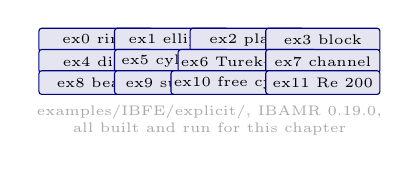
\begin{tikzpicture}[scale=0.6, every node/.style={font=\tiny}]
  \foreach \i/\t in {0/ex0 ring, 1/ex1 ellipse, 2/ex2 plate, 3/ex3 block, 4/ex4 disc, 5/ex5 cylinder, 6/ex6 Turek--Hron, 7/ex7 channel, 8/ex8 beam, 9/ex9 surface, 10/ex10 free cylinder, 11/ex11 Re 200} {
    \node[draw=NavyBlue,fill=NavyBlue!10,rounded corners=1pt,minimum width=1.45cm,minimum height=0.3cm,inner sep=1pt] at ({mod(\i,4)*1.6}, {-floor(\i/4)*0.45}) {\t};
  }
  \node[text=DarkGray,align=center] at (2.4,-1.7) {\code{examples/IBFE/explicit/}, IBAMR 0.19.0,\\ all built and run for this chapter};
\end{tikzpicture}}
\end{frame}

% 2
\begin{frame}{Learning goals}
\label{fr:goals}
\footnotesize By the end of this chapter you should be able to:
\begin{enumerate}
  \item say, for each of IBAMR's twelve finite-element examples, what body is in it, what drives it, what it measures, and which published test it reproduces;
  \item build any of them outside IBAMR's tree with the six-line \code{CMakeLists.txt} and run it on a laptop, and know which ones are smoke tests as shipped (one hundred steps) and which are benchmarks of half an hour to half a day;
  \item recognize the four mechanisms they add to Part IV's: a surface mesh with its own method, a tether that reads fields from another mesh, rigid-body motion by direct forcing, and a stabilized nearly incompressible beam;
  \item read the \code{.curve} files they write (volume, drag and lift, a tip's position, a centre's path) and the MATLAB script that turns lift into a Strouhal number;
  \item know which examples stop as shipped with IBAMR 0.19.0 and why (\code{ex9} on a mesh-dimension assertion; \code{ex5} and \code{ex6} on the ``time step size change'' abort), what that abort means, and what makes the two of them run;
  \item pick the example to start from for a problem of your own, and the chapter of this series that explains its mechanism.
\end{enumerate}
\begin{punchbox}
\scriptsize Chapter 15 toured the point-method examples and ran forty of them; this chapter does the same for the finite-element ones, which chapter 15's map had wrong (slide \ref{fr:correction}).
\end{punchbox}
\end{frame}

% 3
\begin{frame}{Where this chapter comes from}
\label{fr:sources}
\scriptsize
\begin{itemize}
  \item \al{``6 -- IBFE -- What do Boyce's examples do?'' (2020; 19 slides; \code{IBFE\_Lecture\_6}):} a tips slide (Makefile and script per folder, ``timestep size change encountered'', the convergence testers), one slide for each of \code{ex0}--\code{ex8}, \code{ex10} and \code{ex11} with the lecturer's reading of what it does (``I believe'', ``I think'' in several), three figure crops from Griffith and Luo (2017) for \code{ex1}, \code{ex4}, \code{ex5}, and two slides on the complex-fluids examples (``I could not get the examples with immersed boundaries to work (yet)''). No slide for \code{ex9}.
  \item \al{The 2013 lists:} the \emph{IBFE-VisIt} notes and the MATH 769 IBFE deck listed the examples of the day (then \code{ex0}--\code{ex5}); chapter 17 quoted the 2014 getting-started deck's list.
  \item \al{IBAMR 0.19.0:} the twelve \code{example.cpp} files and their inputs, the READMEs of \code{ex5}, \code{ex10} and \code{ex11}, and \code{complex\_fluids/ex2} and \code{ex4}; \code{IBFEMethod.cpp} for the assertion that stops two of them.
  \item \al{The runs:} every example built standalone against 0.19.0 and run on four cores, as shipped and, where the shipped input is a hundred-step smoke test, twenty times longer; the 3D inputs; the two complex-fluid examples with bodies. Report lines in \code{wsl/final/run\_ibfe\_tour.sh}'s output; pictures by \code{wsl/final/visit\_ibfe\_tour.sh}.
  \item \al{New here:} the identification of each example from its code (\code{ex6} is the Turek--Hron benchmark, \code{ex8} a clamped beam over a slot, \code{ex2} not porous); the run table; the three examples that do not run as shipped, why, and what makes two of them run; the complex-fluids examples' one-rank condition; the correction of chapter 15's map; the mechanisms table; own renders in place of the figure crops.
\end{itemize}
\end{frame}

% 4
\begin{frame}{The map (1): \code{ex0} to \code{ex5}}
\label{fr:map}
\scriptsize
\setlength{\tabcolsep}{3pt}
\begin{tabular}{@{}L{0.05\textwidth}L{0.3\textwidth}L{0.3\textwidth}L{0.3\textwidth}@{}}
\toprule
& the body and what drives it & what it tests or measures & chapter here \\
\midrule
ex0 & an elastic ring (radius $0.25$, thickness $0.0625$) at rest in a periodic $1\times1$ box, with the exact pressure jump set as the initial pressure & a static equilibrium: the fluid should stay at rest and the ring's area constant (\code{volume.curve}); the ``sharp'' and ``smooth'' pressure cases & 17 (the mapping), 19 \\
ex1 & the same ring started as an ellipse ($\gamma = 0.15$) in a fluid of viscosity $10^{-2}$ & the dynamic shell test of Griffith and Luo, their Fig.\ 4, $0 \le t \le 0.75$ & 19 \\
ex2 & a soft plate ($\mu = 10$, $0.1$ wide, full height) across a $2\times1$ box; normal stress $-0.1$ on the left face and $+0.1$ on the right & a body pushed by a traction difference with no tether; also in 3D & 22 (boundary conditions) \\
ex3 & a soft block ($c_1 = 0.05$) on the floor of a $2\times2$ cavity whose lid moves at $0.5$ & a solid deformed by a shear flow; the lid velocity is smoothed to zero at the corners & 19 \\
ex4 & a soft disc (radius $0.2$, $c_1 = 0.05$) at $(0.6, 0.5)$ in a $1\times1$ lid-driven cavity, lid speed $1$ & Griffith and Luo's Fig.\ 10 ($3 \le t \le 7$); \code{volume.curve}; a stabilization $\beta$ scaled with the grid; also in 3D & 19 \\
ex5 & a cylinder (radius $0.5$) in a $16\times16$ box at $\mathrm{Re} = 200$, inflow ramped by $\tanh$ with a decaying transverse perturbation & vortex shedding, $C_D$ and $C_L$ (their Fig.\ 12); as a surface mesh with \code{IBFESurfaceMethod} or as a solid disc with body tethers; also in 3D; aborts as shipped (slide \ref{fr:dt}) & 21, 23 \\
\bottomrule
\end{tabular}
\end{frame}

% 4b
\begin{frame}{The map (2a): \code{ex6} to \code{ex8}}
\label{fr:map2a}
\scriptsize
\setlength{\tabcolsep}{3pt}
\begin{tabular}{@{}L{0.05\textwidth}L{0.3\textwidth}L{0.3\textwidth}L{0.3\textwidth}@{}}
\toprule
& the body and what drives it & what it tests or measures & chapter here \\
\midrule
ex6 & a rigid disc (radius $0.05$ at $(0.2, 0.2)$) with an elastic beam ($0.35\times0.02$) behind it in a $2.46\times0.41$ channel; parabolic inflow of mean $2$ ramped over $2$ s; $\rho = 10^3$, $\nu = 10^{-3}$, $\mu_s = 2\times10^6$, $\nu_s = 0.4$ & the Turek--Hron FSI3 benchmark: the beam tip's path (\code{A\_x.curve}, \code{A\_y.curve}), $C_D$, $C_L$; aborts as shipped (slide \ref{fr:dt}) & 21 \\
ex7 & the collapsible channel & chapter 23 in full & 23 \\
ex8 & two rigid blocks with a slot between them and a thin elastic beam ($1\times0.032$) clamped over the slot; a pressure of $80$, ramped over $2$ s, pushes fluid up through the slot & the beam's deformed length and the flux through the slot; a nearly incompressible beam with a grid-scaled stabilization; Chebyshev-spaced beam nodes & 19, 21 \\
\bottomrule
\end{tabular}
\end{frame}

% 4b2
\begin{frame}{The map (2b): \code{ex9} to \code{ex11}}
\label{fr:map2}
\scriptsize
\setlength{\tabcolsep}{3pt}
\begin{tabular}{@{}L{0.05\textwidth}L{0.3\textwidth}L{0.3\textwidth}L{0.3\textwidth}@{}}
\toprule
& the body and what drives it & what it tests or measures & chapter here \\
\midrule
ex9 & a cylinder's \emph{boundary} mesh tethered, in position and velocity, to fields on the solid mesh (at rest as shipped) in a tall still box & a template for a surface tethered to a prescribed motion; stops at once in 0.19.0 (slide \ref{fr:fail}) & 21 \\
ex10 & a neutrally buoyant rigid cylinder (diameter $1$) free to move in a plane Couette flow (walls at $\pm1$, channel $4$ high, $160$ long, periodic) at $\mathrm{Re} = 40$ & inertial migration of a free body; the centre's path and velocity (\code{X.curve}, \code{U.curve}); direct forcing of a rigid body & this chapter \\
ex11 & a fixed rigid cylinder (radius $0.5$) at $\mathrm{Re} = 200$ in a $32\times16$ box, ramped inflow with a perturbation & $C_D$, $C_L$ and the Strouhal number (\code{compute\_St.m}); direct forcing & this chapter \\
\bottomrule
\end{tabular}
\end{frame}

% 4c
\begin{frame}{The map (3): what chapter 15 said, and the correction}
\label{fr:correction}
\footnotesize
\begin{itemize}
  \item Chapter 15's slide 31 (``\code{IBFE/explicit}: twelve examples for Part IV'') gave a one-line map that was wrong: it listed this series' own examples (the rotated plate, the active tension, the plate that hits the disc, the flow tank, the scalar) under IBAMR's numbers. The slide is corrected in the current build to the map of slides \ref{fr:map}--\ref{fr:map2}; if your copy says ``ex6 a contracting body with an active stress'', it is the old one.
  \item The 2020 lecture's own readings, checked against the code: \code{ex0} ``tests the conservation of volume in the shell'' (right: \code{volume.curve}); \code{ex2} ``porous FE boundaries \ldots the first example'' (no: a soft plate pushed by a traction difference; there is no porosity in the code); \code{ex6} ``I believe it comes from a paper by Boyce, but I have not found it yet'' (it is Turek and Hron's 2006 benchmark, the FSI3 parameters); \code{ex7} ``I believe this is an example of peristaltic transport'' (a collapsible channel, chapter 23); \code{ex8} ``two solid blocks with a rigid, porous plate on top'' (an elastic beam clamped over a slot, not rigid, not porous).
  \item ``I believe'' and ``I think'' were the right words in 2020; the code and the runs replace them here.
\end{itemize}
\end{frame}

% 5
\begin{frame}{Building and running them (1): 2020}
\label{fr:build2020}
\footnotesize
2020 (slide 3, ``Tips for running examples''): ``Remember to move a Makefile and script.sh to each folder. Make sure the Makefile has the right dimensions, make sure the script.sh uses the right input file. Some of the examples go unstable (timestep size change encountered). Just reduce DT in the input file and rerun. Some of the examples have other .C or .cpp files for convergence tests, etc.\ The Makefile we use compiles all .C files in the folder. Drop the .C / .cpp and then make.''
\begin{itemize}
  \item Every point survives in a new form: the dimension is the CMake target (\code{IBAMR2d} or \code{3d}), the input file is the argument, the time-step abort is slide \ref{fr:dt} (where ``just reduce DT'' is tried on the two examples that abort, and is not enough), and the extra files are the ones the CMake list leaves out.
  \item The 2020 course ran them in IBAMR's tree with the course Makefile (chapter 15's first route). The examples are the same twelve today, with the same inputs; the tip about instability was written because two of them aborted then as they do now.
\end{itemize}
\end{frame}

% 5a
\begin{frame}[fragile]{Building and running them (2): now}
\label{fr:build}
\footnotesize
Chapter 15's second route; \code{wsl/final/run\_ibfe\_tour.sh} does this for all of them:
\begin{lstlisting}[style=shell]
cp -r $IBAMR_SRC/examples/IBFE/explicit/ex4 ex4 && cd ex4
rm CMakeLists.txt Makefile.am Makefile.in     # the in-tree build files
cat > CMakeLists.txt <<EOF
cmake_minimum_required(VERSION 3.15...3.30)
project(ex4 LANGUAGES C CXX)
find_package(IBAMR 0.16.0 REQUIRED)
add_executable(main2d example.cpp)           # not convergence_tester.cpp
target_link_libraries(main2d PRIVATE IBAMR::IBAMR2d)
EOF
cmake -S . -B build -DCMAKE_BUILD_TYPE=Release && cmake --build build -j 4
mpirun -np 4 ./build/main2d input2d          # or main3d input3d
\end{lstlisting}
\begin{itemize}
  \item \code{ex4} and \code{ex5} carry a \code{convergence\_tester.cpp}; \code{ex7} three inputs (\code{caseC}, \code{caseS2}, \code{caseSP}); \code{ex2}, \code{ex4}, \code{ex5}, \code{ex9} an \code{input3d} as well. Build time is $30$--$50$ s each on the laptop.
\end{itemize}
\end{frame}

% 5b
\begin{frame}{Building and running them (3): how long they are}
\label{fr:length}
\footnotesize
\begin{itemize}
  \item \al{Smoke tests as shipped.} \code{ex0}--\code{ex6} and \code{ex8} have \code{END\_TIME = 100*DT}: one hundred steps, a few seconds, enough to see that the program builds and the first frames look right, not enough to see the physics. \code{ex7} has $1000$ steps. The run table (slide \ref{fr:table}) gives each one's hundred steps in physical time.
  \item \al{Benchmarks.} \code{ex9} runs to $t = 15$, \code{ex11} to $130$ (65\,000 steps on a $1024\times512$ fine grid), \code{ex10} to $1200$ (240\,000 steps): ``This is a long simulation with many file writes'' (2020, slides 15--16). These are the ones with \code{.curve} output meant to be compared with published numbers.
  \item For the pictures of this chapter, the smoke tests were rerun twenty times longer (\code{END\_TIME = 2000*DT}) under a fifteen-minute cap, and the benchmarks for half an hour each; the tables say how far each got: \code{ex11} to the end of its $130$ time units, \code{ex10} to $52$ of $1200$. Chapter 16's rule applies before any of them is trusted: refine and compare.
  \item The three Griffith and Luo figures the 2020 deck cropped (\code{ex1}'s shell, \code{ex4}'s disc, \code{ex5}'s cylinder) are replaced here by renders of the runs (slides \ref{fr:gallery}--\ref{fr:gallery2}); the paper is the reference for the numbers.
\end{itemize}
\end{frame}

% 6
\begin{frame}[fragile]{\code{ex0} and \code{ex1} (1): the ring's code}
\label{fr:ex01}
\footnotesize
\begin{columns}[T]
\column{0.55\textwidth}
\begin{lstlisting}[style=cpptiny]
static const double R = 0.25;       // the ring's inner radius
static const double w = 0.0625;     // its thickness
static const double gamma = 0.0;    // ex1: 0.15, an ellipse
static const double mu = 1.0;
void coordinate_mapping_function(libMesh::Point& X, const libMesh::Point& s, void* /*ctx*/)
{
    X(0) = (R + s(1)) * cos(s(0) / R) + 0.5;            // s(0): arc length round the ring
    X(1) = (R + gamma + s(1)) * sin(s(0) / R) + 0.5;   // s(1): across the thickness
}
void PK1_stress_function(...) { PP = (mu / w) * FF; ... }
\end{lstlisting}
\column{0.43\textwidth}
\begin{itemize}
  \item The mesh is a rectangle ($2\pi R$ by $w$, \code{QUAD9}, \code{MFAC = 4}) that chapter 17's coordinate mapping bends into a ring: $s_0$ is the arc length, $s_1$ the position across the thickness.
  \item The stress $\mu\mathbb{F}/w$ is a membrane tension spread over the thickness: the simplest stress of chapter 19, with no resistance to compression or shear beyond the fluid's.
  \item One file serves both examples: \code{gamma} is the only difference, and the input's \code{MU} and viscosity change with it.
\end{itemize}
\end{columns}
\end{frame}

% 6b
\begin{frame}[fragile]{\code{ex0} and \code{ex1} (2): the test at rest, and the ellipse}
\label{fr:ex01b}
\footnotesize
\begin{lstlisting}[style=inputtiny]
SMOOTH_CASE = FALSE
PressureInitialConditions {
   p0_smooth = (mu*PI/(3*w))*(R^2 - (R+w)^3/R)
   p0_sharp = mu*PI*R
   function = "(sqrt((X0-0.5)^2 + (X1-0.5)^2) < R ? (p0_sharp - mu/(R+w)) : ...)"
}
\end{lstlisting}
\begin{itemize}
  \item \code{ex0}: ``This is a pressurized shell, the colormap shows the pressure. There is no significant fluid motion'' (2020, slide 4). The input sets the \emph{exact} pressure jump of the ring in equilibrium as the initial pressure (two formulas, for a tension spread smoothly or sharply across $w$); the fluid should then stay at rest, and \code{volume.curve} should stay flat. It is the first test of Griffith and Luo's paper.
  \item \code{ex1}: $\gamma = 0.15$ makes the ring an ellipse ($0.25$ by $0.40$ in radius) in a fluid of viscosity $10^{-2}$; it relaxes toward a circle and overshoots. ``This example comes from Figure 4, Griffith and Luo: representative results from the dynamic ($\gamma = 0.15$) version of the idealized anisotropic shell model of Section 5.1.1 for $N = 128$ over $0 \le t \le 0.75$'' (slide 6). As shipped it stops at $t = 0.2$; the longer run (slide \ref{fr:table2}) reaches $t = 3.9$.
\end{itemize}
\end{frame}

% 7
\begin{frame}{\code{ex2}, \code{ex3}, \code{ex4}: soft bodies pushed by boundary conditions}
\label{fr:ex234}
\scriptsize
\begin{itemize}
  \item \al{\code{ex2}.} A $2\times1$ box with no periodic sides and a plate $0.1$ thick spanning its full height at $x = 1$ (\code{build\_square} from $0.95$ to $1.05$); neo-Hookean $\mu = 10$ (the \code{mu*FF} and \code{-mu*FF\^{}\{-T\}} pair of chapter 19); no tether. The $x$-velocity's boundary condition on the left and right faces is a \emph{traction} ($a = 0$, $b = 1$): $-0.1$ on the left, $+0.1$ on the right, a normal-stress difference of $0.2$ across the box that pushes fluid, and the plate with it. The 2020 reading, ``porous FE boundaries \ldots The porous plate takes up the entire channel, and flow is driven through it'', is half right: the plate takes up the channel and the boundary conditions drive the flow, but the code has no porosity, and what goes through the plate goes through because the IB kernel lets the grid's fluid leak through a soft body held by nothing: the test is of that leak. Three levels, $\mathrm{DX} = 1/64$. Also in 3D.
  \item \al{\code{ex3}.} ``Cavity driven flow with a flexible material on the bottom'' (slide 8): a $2\times0.5$ block on the floor of a $2\times2$ cavity, \code{QUAD9}, $c_1 = 0.05$ ($\mathbb{P} = 2c_1\mathbb{F}$, the neo-Hookean form written with $c_1 = \mu_s/2$), the lid moving at $0.5$ with $\sin^2$ ramps to zero over $0.3$ at the two corners so that the corner singularity of the classic cavity is avoided. Two levels, $\mathrm{DX} = 1/32$.
  \item \al{\code{ex4}.} ``A soft neo-Hookean disc in a lid-driven cavity flow using the partitioned (split) weak formulation with $N = 128$ and $\mathrm{Mfac} = 4$ over $3 \le t \le 7$'' (slide 9, from Griffith and Luo's Fig.\ 10): a disc of radius $0.2$ built by \code{build\_sphere} with \code{TRI6}, its boundary nodes snapped onto the exact circle, mapped to $(0.6, 0.5)$; lid speed $1$; $c_1 = 0.05$ and a dilatational stabilization $\beta_s = \mathrm{NFINEST}/64$ that grows with the grid; \code{volume.curve}. The shipped input is $N = 64$, one level, one hundred steps ($t = 0.1$): ``This example only runs for two data visualization writes. You can increase the endtime to run for longer'' (slide 10). Also in 3D (a sphere).
\end{itemize}
\end{frame}

% 8
\begin{frame}[fragile]{\code{ex5} (1): the cylinder at $\mathrm{Re} = 200$, as a surface or a solid}
\label{fr:ex5}
\footnotesize
\begin{lstlisting}[style=cpptiny]
BoundaryMesh boundary_mesh(solid_mesh.comm(), solid_mesh.mesh_dimension() - 1);
solid_mesh.boundary_info->sync(boundary_mesh);
boundary_mesh.prepare_for_use();
bool use_boundary_mesh = input_db->getBoolWithDefault("USE_BOUNDARY_MESH", false);
Mesh& mesh = use_boundary_mesh ? boundary_mesh : solid_mesh;
...   // IBFESurfaceMethod for the boundary mesh, IBFEMethod for the solid
F = tether_data->kappa_s_surface * D - tether_data->eta_s_surface * U;   // the surface tether
PP = 2.0 * tether_data->c1_s * (FF - tensor_inverse_transpose(FF, NDIM));  // the solid's penalty stress
\end{lstlisting}
\begin{lstlisting}[style=inputtiny]
Re = 200.0
USE_BOUNDARY_MESH = TRUE
MAX_LEVELS = 6   N = 16   L = 16.0   MFAC = 8.0   ELEM_TYPE = "TRI6"
KAPPA_S_SURFACE = 1.0e6   ETA_S_SURFACE = 0.0   C1_S = 1.0e5
VelocityBcCoefs_0 { t_half = 0.5  tau = 0.125
   gcoef_function_0 = "(tanh((t-t_half)/tau)+tanh(t_half/tau))/(1+tanh(t_half/tau))" }
VelocityBcCoefs_1 { gcoef_function_0 = "cos(pi*X_1/16.0)*exp(-2.0*t)" }
\end{lstlisting}
\begin{itemize}
  \item ``From Figure 12, Griffith and Luo: vortices shed from a stationary circular cylinder at $\mathrm{Re} = 200$'' (slide 11). Radius $0.5$ in a box $-8 < x < 24$, $-8 < y < 8$; six levels on a $16$-cell base ($\mathrm{DX} = 1/32$ at the cylinder); the inflow ramped by the same $\tanh$ as chapter 22's crab, plus a transverse velocity $\cos(\pi y/16)\,e^{-2t}$ at the inflow face that dies in a few time units: the nudge that starts the shedding on a symmetric grid.
\end{itemize}
\end{frame}

% 8b
\begin{frame}{\code{ex5} (2): two bodies in one file, and what happened}
\label{fr:ex5b}
\footnotesize
\begin{itemize}
  \item \al{Two bodies in one file.} \code{USE\_BOUNDARY\_MESH = TRUE} (the shipped choice): the cylinder is its boundary curve only, extracted from the disc by libMesh's \code{BoundaryMesh}, handled by \code{IBFESurfaceMethod}, and held by a surface tether $\kappa_s(\mathbf{X}_0 - \mathbf{X}) - \eta_s\mathbf{U}$. \code{FALSE}: the solid disc with \code{IBFEMethod}, a body tether and a penalty stress $c_1 = 10^5$. Chapter 21's parts, chapter 19's surface forces, and a thin-surface method this series has not needed.
  \item Output: \code{C\_D.curve}, \code{C\_L.curve}, \code{U\_max.curve}. ``I had some issues reading the .ex2 file for this. It looks like ex11 is a very similar example which does run well'' (slide 11). Also in 3D (a sphere).
  \item \al{What happened.} As shipped, in 2D and in 3D, the run aborts after five steps with \code{Time step size change encountered}; with \code{DT} halved, after eleven. Slide \ref{fr:dt} follows this up: the step is not the problem, the surface tether is.
\end{itemize}
\end{frame}

% 9
\begin{frame}[fragile]{\code{ex6} (1): the Turek--Hron beam behind a cylinder}
\label{fr:ex6}
\footnotesize
\begin{columns}[T]
\column{0.5\textwidth}
\begin{lstlisting}[style=inputtiny]
L     = 2.46          // channel length
H     = 0.41          // channel height
RHO   = 1.0e3
NU    = 1.0e-3
MU    = RHO*NU
U_BAR = 2.0           // mean inflow speed
D     = 0.1           // cylinder diameter
RE    = U_BAR*D*RHO/MU          // 200
MU_S = 2.0e6          // the beam's shear modulus
NU_S = 0.4
LAMBDA_S = 2.0*MU_S*NU_S/(1.0 - 2.0*NU_S)
KAPPA_S = 2*2.5e4 * DX / DT^2   // the block's tether
VelocityBcCoefs_0 { U_bar = U_BAR  H = H
   gcoef_function_0 = "1.5*U_bar*X1*(H-X1)/((H/2)^2)*(t < 2.0 ? 0.5*(1.0-cos(0.5*pi*t)) : 1.0)" }
\end{lstlisting}
\column{0.48\textwidth}
\begin{lstlisting}[style=cpptiny]
MeshTools::Generation::build_sphere(block_mesh, R, r, ...);   // then shifted to (0.2, 0.2)
MeshTools::Generation::build_square(beam_mesh, ceil(0.4 / ds), ceil(0.02 / ds), 0.2, 0.6, 0.19, 0.21, ...);
vector<MeshBase*> meshes(2);  meshes[0] = &block_mesh;  meshes[1] = &beam_mesh;
// the beam's tether holds only its part inside the disc:
const double r = sqrt((s(0) - 0.2) * (s(0) - 0.2) + (s(1) - 0.2) * (s(1) - 0.2));
if (r <= 0.05) F = elasticity_data->kappa_s * (s - X); else F.zero();
\end{lstlisting}
\footnotesize The input is in SI units, the only example of the twelve that is: a channel $2.46$ m long, water-like $\rho$ and $\nu$, a mean inflow of $2$ m/s, and a beam of shear modulus $2$ MPa. Chapter 8a's rule (regenerate the stiffnesses when the grid or the step changes) is built into \code{KAPPA\_S}.
\end{columns}
\end{frame}

% 9b
\begin{frame}{\code{ex6} (2): the benchmark, the two parts, and what happened}
\label{fr:ex6b}
\footnotesize
\begin{itemize}
  \item ``A standard example of a relatively rigid circle attached to a flexible plate that bends as vortices are shed. I believe it comes from a paper by Boyce, but I have not found it yet'' (slide 12). It is the Turek--Hron FSI benchmark (2006), case FSI3: channel $2.5\times0.41$ (here $2.46$), cylinder of diameter $0.1$ at $(0.2, 0.2)$, beam $0.35\times0.02$ behind it, $\rho_f = \rho_s = 10^3$, $\nu = 10^{-3}$, $\bar U = 2$ m/s, $\mu_s = 2\times10^6$ Pa, $\nu_s = 0.4$, the inflow parabola ramped over $2$ s with $\tfrac12(1 - \cos\tfrac{\pi t}{2})$: every number is the benchmark's.
  \item Two parts (chapter 21): the disc, held rigid by a tether and a penalty stress; the beam, St.\ Venant--Kirchhoff with $\mu_s$, $\lambda_s$, built $0.4$ long so that its root sits inside the disc, where the same tether clamps it. The \code{ctx} pointer carries the constants into the callbacks (chapter 19).
  \item Output: the beam tip A at $(0.6, 0.2)$ in \code{A\_x.curve}, \code{A\_y.curve}, and $C_D$, $C_L$. FSI3's published tip oscillation: amplitude about $0.034$ in $y$ at $5.3$ Hz. As shipped: four levels on an $8$-cell base ($\mathrm{DX} = 0.038$), one hundred steps.
  \item \al{What happened.} As shipped the run aborts after fourteen steps ($t = 0.004$ s, before the inflow ramp has reached a hundredth of its value) with \code{Time step size change encountered}; slide \ref{fr:dt}.
\end{itemize}
\end{frame}

% 10
\begin{frame}[fragile]{\code{ex8} (1): a clamped beam over a slot}
\label{fr:ex8}
\footnotesize
\begin{lstlisting}[style=cpptiny]
build_square(block1_mesh, ..., 0.0, 0.5, 0.0, 0.5, ...);   // two rigid blocks
build_square(block2_mesh, ..., 1.5, 2.0, 0.0, 0.5, ...);
const double beam_x_lower = 0.5, beam_x_upper = 1.5;     // the beam spans the slot
const double beam_y_lower = 0.5 - 0.016;                 // 0.032 thick
build_square(beam_mesh, n_beam_x, n_beam_y, beam_x_lower, beam_x_upper, beam_y_lower, beam_y_upper, QUAD4);
if (beam_use_mapped_grid) { ... cheby(...) ... }         // Chebyshev-spaced nodes, finer near the ends
// the beam's tether acts on its two ends only (a surface force on sides 1 and 3):
if (side == 1 || side == 3) F = beam_kappa_s * (s - X); else F.zero();
PP = mu_s * (FF - FF_inv_trans);  // plus a beta_s log(J) term when BETA_S != 0
\end{lstlisting}
\begin{lstlisting}[style=inputtiny]
MU_S = 1.0e3   P_MAX = 80.0   T_END = 2.0
BETA_S = SAFETY * 1.25e-2 * MU_S / sqrt(DT)
BEAM_KAPPA_S = SAFETY * 5.0e1 * DX / DT^2
VelocityBcCoefs_1 {   // the bottom face, between the blocks: a pressure, ramped
   acoef_function_2 = "(X_0 > 0.5) && (X_0 < 1.5) ? 0.0 : 1.0"
   bcoef_function_2 = "(X_0 > 0.5) && (X_0 < 1.5) ? 1.0 : 0.0"
   gcoef_function_2 = "(X_0 > 0.5) && (X_0 < 1.5) ? -p_max * min(1.0, t/t_end) : 0.0" }
\end{lstlisting}
\begin{itemize}
  \item The boundary condition on the bottom face is written per point: Dirichlet ($a = 1$) outside the slot, a normal traction ($b = 1$) that ramps to $-80$ inside it. Chapter 22's recipe for a mixed face in one expression.
\end{itemize}
\end{frame}

% 10b
\begin{frame}{\code{ex8} (2): what it is, and what to copy}
\label{fr:ex8b}
\footnotesize
\begin{itemize}
  \item ``The second example of possible porous boundaries in IBAMR. The example consists of two solid blocks with a rigid, porous plate on top. Flow is driven from the bottom of the domain through the porous plate'' (slide 14). The code: two blocks $0.5\times0.5$ held rigid by body tethers, a beam $1$ long and $0.032$ thick spanning the slot between them, clamped at its two ends by a \emph{surface} tether (chapter 19, slide 24; chapter 21's ex8 pattern), and a pressure of $80$ applied on the bottom face under the slot, ramped over $2$ s: the fluid is pushed up through the slot and bows the beam. Neither rigid nor porous: an elastic beam, $\mu_s = 10^3$, nearly incompressible, with a stabilization $\beta_s \propto \mu_s/\sqrt{\mathrm{DT}}$.
  \item \al{Two things to copy:} the Chebyshev spacing of the beam's nodes (finer at the clamped ends, where the bending is), and the post-processing: the beam centre line's deformed length and the flux through the slot (\code{compute\_deformed\_length}, \code{compute\_inflow\_flux}), the latter a loop over the patches touching the bottom face.
  \item Shipped: $N = 48$, one level, one hundred steps ($t = 0.04$, before the ramp has done anything); the longer run (slide \ref{fr:table2}) shows the bow.
\end{itemize}
\end{frame}

% 11
\begin{frame}[fragile]{\code{ex10} and \code{ex11} (1): rigid bodies by direct forcing}
\label{fr:ex1011}
\footnotesize
\begin{lstlisting}[style=cpptiny]
#include <ibamr/IBFEDirectForcingKinematics.h>
void cylinder_kinematics(double /*data_time*/, Eigen::Vector3d& U_com, Eigen::Vector3d& W_com, void* /*ctx*/)
{   U_com.setZero();  W_com.setZero(); }        // the prescribed part of the motion: none
...
Pointer<IBFEDirectForcingKinematics> df_kinematics_ops = new IBFEDirectForcingKinematics(
    "cylinder_dfk", app_initializer->getComponentDatabase("CylinderIBFEDirectForcingKinematics"), ib_method_ops, /*part*/ 0);
ib_method_ops->registerDirectForcingKinematics(df_kinematics_ops, /*part*/ 0);
df_kinematics_ops->setSolveRigidBodyVelocity(solve_dofs);     // ex10: which of the body's six degrees of freedom are free
df_kinematics_ops->registerKinematicsFunction(&cylinder_kinematics, nullptr);
\end{lstlisting}
\begin{itemize}
  \item \al{The mechanism.} \code{IBFEDirectForcingKinematics} makes a part rigid without tethers: each step it computes the fluid force on the body, advances the body's rigid translation and rotation (for the degrees of freedom that are free), and then forces the body's velocity onto the fluid. The kinematics function supplies the \emph{prescribed} part (zero here); \code{setSolveRigidBodyVelocity} says which components are solved for. The part's finite element mesh is only a shape.
  \item Compare chapter 14's constraint IB (the same idea for point bodies: compute the force, move the body, impose its velocity) and chapter 20's targets (a soft version: the body is pulled, not set).
\end{itemize}
\end{frame}

% 11b
\begin{frame}[fragile]{\code{ex10} (2): a free cylinder in a Couette flow}
\label{fr:ex10}
\footnotesize
\begin{lstlisting}[style=inputtiny]
R = 0.5   D = 2*R   H = 4*D   L = 40*H   Uw = 1.0   Re = 40.0
MU = 2.0*RHO*Uw*H/Re
CylinderIBFEDirectForcingKinematics { rho_s = RHO }   // neutrally buoyant
VelocityBcCoefs_0 { gcoef_function_2 = "U_wall"  gcoef_function_3 = "-U_wall" }
periodic_dimension = 1,0
\end{lstlisting}
\begin{itemize}
  \item \al{\code{ex10}} (README: ``FSI of cylinder in a shear-driven channel flow at $\mathrm{Re} = 40$''): a neutrally buoyant cylinder of diameter $1$ in a channel $4$ high and $160$ long, periodic in $x$, with the walls moving at $+1$ and $-1$: a plane Couette flow. The cylinder is free, and its centre's path (\code{X.curve}) and velocity (\code{U.curve}) show it migrate to the centre line, the classic inertial-migration result for a free body in a shear flow. ``This is a long simulation with many file writes'' (slide 15): \code{END\_TIME = 1200}.
  \item \al{What happened.} On four cores the shipped run reaches $t = 28$ in fifteen minutes (slide \ref{fr:table}); \code{X.curve} and \code{U.curve} have the centre's path to there. The migration takes hundreds of time units: exercise 6.
\end{itemize}
\end{frame}

% 11c
\begin{frame}[fragile]{\code{ex11} (3): the fixed cylinder at $\mathrm{Re} = 200$ by direct forcing}
\label{fr:ex11}
\footnotesize
\begin{lstlisting}[style=inputtiny]
Re = 200.0   N = 256   MAX_LEVELS = 2   REF_RATIO = 4   DT = 0.002   END_TIME = 130.0
x_lo = -8.0, -8.0   x_up = 24.0, 8.0
\end{lstlisting}
\begin{itemize}
  \item \al{\code{ex11}} (README: ``flow past cylinder using IBFEDirectForcingKinematics at $\mathrm{Re} = 200$''): the fixed-cylinder benchmark of \code{ex5} done with a rigid body instead of tethers, on a $256\times128$ base with one refinement; $C_D$, $C_L$ to \code{.curve} files and \code{compute\_St.m}, which finds the Strouhal number from the lift by a Fourier transform and by zero crossings (published: $\mathrm{St} \approx 0.19$--$0.20$, $C_D \approx 1.3$--$1.4$ at $\mathrm{Re} = 200$). \code{END\_TIME = 130}.
  \item \al{What happened.} It runs as shipped, and fast: the whole benchmark, $65\,000$ steps to $t = 130$, took $27$ minutes on four cores (slide \ref{fr:table2}), writing $651$ frames; the gallery shows its wake. ``Long'' in 2020 was the course cluster's queue, not the problem. The \code{ex5} ``.ex2 read issue'' of 2020 that sent the lecturer here does not arise with VisIt 3.5.
\end{itemize}
\end{frame}

% 12
\begin{frame}{\code{ex9}, and the ones that stop as shipped}
\label{fr:fail}
\footnotesize
\begin{itemize}
  \item \al{\code{ex9}} has no 2020 slide. Its code: a cylinder's \emph{boundary mesh} (libMesh's \code{BoundaryMesh} of a disc, one-dimensional elements in a two-dimensional box) is the IB body, tethered to two fields defined on the \emph{solid} disc, a ``position'' and a ``velocity'' system, with $\mathbf{F} = \kappa_s(\mathbf{x}_{\mathrm{solid}} - \mathbf{x}) + \eta_s(\mathbf{u}_{\mathrm{solid}} - \mathbf{u})$; the callback finds the solid element under each boundary element with \code{interior\_parent()}. As shipped the position field is the rest shape and the velocity zero, the box ($16\times32$, traction-free sides, no inflow) is still, and nothing happens: the file is a template for a surface that follows a motion defined on a volume, with both a position and a velocity penalty, not a flow problem. Its \code{// \textbackslash todo} says so: ``There needs to be an API so that this can be handled by the IBFEMethod class implementation.''
  \item \al{Why it stops now.} Built and run against 0.19.0 it aborts before the first step:
\end{itemize}
\begin{center}\scriptsize\code{Failed assertion: mesh->mesh\_dimension() == mesh->spatial\_dimension()} \quad (\code{IBFEMethod.cpp}, line 376)\end{center}
\begin{itemize}
  \item \code{IBFEMethod} now accepts only meshes of the box's dimension (areas in 2D, volumes in 3D); a curve in 2D or a surface in 3D goes to \code{IBFESurfaceMethod} (what \code{ex5} switches to for its boundary mesh) or to the \code{IIM} suite. Chapter 15 met the same assertion in \code{IBLevelSet/ex0}. \code{ex9}'s 3D input stops the same way.
  \item \al{\code{ex5} (2D and 3D) and \code{ex6}} stop after five and fourteen steps with the other classic message, \code{Time step size change encountered}: slide \ref{fr:dt}.
\end{itemize}
\end{frame}

% 13
\begin{frame}{``Time step size change encountered'' (1): what the message means}
\label{fr:dt}
\footnotesize
\begin{itemize}
  \item The message comes from \code{IBHierarchyIntegrator::preprocessIntegrateHierarchy()} (line 213 in 0.19.0) when \code{error\_on\_dt\_change = TRUE} (every example input sets it through \code{ERROR\_ON\_DT\_CHANGE}) and the step the integrator wants differs from the last one: the CFL limit, computed from the current velocity, has fallen below \code{dt\_max}. The abort is deliberate: a shrinking step means the velocity has grown past what the input assumed, usually the start of an instability, and the examples would rather stop than run on with a step that changes. With \code{error\_on\_dt\_change = FALSE} and \code{warn\_on\_dt\_change = TRUE} the same check prints ``WARNING: Time step size change encountered. Suggest reducing maximum time step size in input file'' and goes on with the smaller step.
  \item ``Some of the examples go unstable (timestep size change encountered). Just reduce DT in the input file and rerun'' (2020, slide 3). Two of the twelve abort as shipped, \code{ex5} after five steps (2D and 3D) and \code{ex6} after fourteen, before either inflow ramp has done anything: whatever grows, grows from rest. The next slide tries the tip and two other things on each.
  \item What the step must satisfy here: the fluid CFL ($U\,\mathrm{DT}/\mathrm{DX} \le$ \code{cfl}); a penalty spring's limit, $\mathrm{DT} \lesssim \sqrt{m/\kappa_s}$ for the mass $m$ a spring moves (chapter 8a's rule: the inputs write $\kappa_s \propto \mathrm{DX}/\mathrm{DT}^2$ \emph{from} the step, so halving \code{DT} quadruples $\kappa_s$ and keeps the ratio); and the elastic wave speed $\sqrt{\mu_s/\rho_s}$ in a stiff body (chapter 16). An input that fixes $\kappa_s$ by hand, as \code{ex5} does, breaks the first rule when the grid or the step changes.
\end{itemize}
\end{frame}

% 13b
\begin{frame}{``Time step size change encountered'' (2): what was tried on \code{ex5} and \code{ex6}}
\label{fr:dt2}
\scriptsize
\setlength{\tabcolsep}{3pt}
\begin{tabular}{@{}L{0.11\textwidth}L{0.37\textwidth}L{0.46\textwidth}@{}}
\toprule
& \code{ex5} (a cylinder surface held by \code{KAPPA\_S\_SURFACE = 1e6}, \code{ETA = 0}) & \code{ex6} (a disc held by \code{KAPPA\_S = 2*2.5e4*DX/DT\^{}2}, a beam of $\mu_s = 2$ MPa) \\
\midrule
as shipped & aborts at step 5 & aborts at step 14 \\
\code{DT} halved (the 2020 tip) & aborts at step 11: the tip only delays it & runs the hundred steps: the tip works \\
the step allowed to change & finishes the shipped run in $1585$ steps instead of $100$: the step falls to a tenth to a thirtieth of \code{DT} and stays there, fluctuating & finishes in $403$ steps: the step settles at about a quarter of \code{DT} \\
the tether changed & the input's own, unused, grid-scaled constants (\code{KAPPA\_S = 2.5*DX/DT\^{}2}, \code{ETA\_S = 1.5*DX/DT}, lines 48--49 of \code{input2d}) in place of the fixed $10^6$ and $0$: runs the hundred steps at the shipped \code{DT}, in $6$ s & a hundred times softer (\code{2*2.5e2}): aborts at step 17 \\
\midrule
reading & the undamped surface spring is thirty times stiffer than the grid-scaled rule allows at this step; the surface rings and the fluid next to it moves at tens of units while the inflow is still zero & the step, not the tether: at the shipped \code{DT} the beam's elastic wave ($\sqrt{\mu_s/\rho_s} \approx 45$ m/s) crosses a third of a cell per step, and the coupled scheme does not tolerate it; half the step does \\
\bottomrule
\end{tabular}

\medskip
The fix for \code{ex5} is in its own input file; the fix for \code{ex6} is the 2020 tip. Letting the step change is a diagnosis, not a fix: it shows how far the step wants to fall, at four to sixteen times the cost.
\end{frame}

% 14
\begin{frame}{The mechanisms these examples add (1)}
\label{fr:mechanisms}
\footnotesize
\setlength{\tabcolsep}{3pt}
\begin{tabular}{@{}L{0.33\textwidth}L{0.14\textwidth}L{0.44\textwidth}@{}}
\toprule
mechanism & where & what it is for \\
\midrule
a surface (codimension-one) body with \code{IBFESurfaceMethod} & \code{ex5} & a thin shell or membrane as a curve or surface mesh, with its own interaction rules; what \code{IBFEMethod} no longer accepts \\
a tether that reads fields from another mesh (\code{interior\_parent}, \code{point\_value}) & \code{ex9} & drive a surface from a motion defined on a volume; a position and a velocity penalty together \\
rigid-body motion by direct forcing (\code{IBFEDirectForcingKinematics}) & \code{ex10}, \code{ex11} & a rigid part without tethers, free or prescribed, with the fluid force integrated for you \\
a stabilized nearly incompressible beam ($\beta_s \propto \mu_s/\sqrt{\mathrm{DT}}$) and Chebyshev node spacing & \code{ex8} & thin elastic structures that must not lose volume \\
\bottomrule
\end{tabular}

\medskip
These four are new to this series; the next slide lists the smaller devices worth copying.
\end{frame}

% 14b
\begin{frame}{The mechanisms these examples add (2): smaller devices}
\label{fr:mechanisms2}
\footnotesize
\setlength{\tabcolsep}{3pt}
\begin{tabular}{@{}L{0.29\textwidth}L{0.15\textwidth}L{0.47\textwidth}@{}}
\toprule
device & where & what it is for \\
\midrule
a penalty stress $c_1(\mathbb{F} - \mathbb{F}^{-T})$ plus a tether for a ``rigid'' part & \code{ex5}, \code{ex6} & a rigid body done with elasticity, the way Part IV did it \\
the exact pressure as an initial condition & \code{ex0} & a static test with a known answer \\
a transverse perturbation at the inflow that decays & \code{ex5}, \code{ex11} & start shedding on a symmetric grid without waiting for round-off \\
constants through \code{ctx} & \code{ex5}, \code{ex6} & chapter 19's way to give callbacks their parameters \\
\bottomrule
\end{tabular}

\medskip
The ones Part IV already used: parts and per-part registration (\code{ex6}--\code{ex8}), the coordinate mapping (\code{ex0}, \code{ex1}, \code{ex4}), body and surface tethers (all), two stress functions (\code{ex2}--\code{ex4}, \code{ex7}, \code{ex8}), the sponge layer (\code{ex7}).
\end{frame}

% 15
\begin{frame}{What was run for this chapter}
\label{fr:table}
\scriptsize
\setlength{\tabcolsep}{3pt}
\begin{tabular}{@{}l l l l r r r L{0.3\textwidth}@{}}
\toprule
example & dim & input & \code{END\_TIME} & steps & time $t$ & wall & outcome \\
\midrule
ex0 & 2D & \code{input2d} & shipped & 100 & 0.195312 & 2 s & ran to the end \\
ex1 & 2D & \code{input2d} & shipped & 100 & 0.195312 & 3 s & ran to the end \\
ex2 & 2D & \code{input2d} & shipped & 100 & 0.390625 & 2 s & ran to the end \\
ex3 & 2D & \code{input2d} & shipped & 100 & 1.875 & 2 s & ran to the end \\
ex4 & 2D & \code{input2d} & shipped & 100 & 0.048828 & 1 s & ran to the end \\
ex5 & 2D & \code{input2d} & shipped & 5 & 0.007812 & 1 s & time-step change abort (slide \ref{fr:dt}) \\
ex6 & 2D & \code{input2d} & shipped & 14 & 0.004035 & 1 s & time-step change abort (slide \ref{fr:dt}) \\
ex7 & 2D & \code{input2d.caseC} & shipped & 1000 & 0.019531 & 33 s & ran to the end \\
ex8 & 2D & \code{input2d} & shipped & 100 & 0.041666 & 1 s & ran to the end \\
ex9 & 2D & \code{input2d} & shipped & 0 & -- & 0 s & mesh-dimension assertion (slide \ref{fr:fail}) \\
ex10 & 2D & \code{input2d} & shipped & 5585 & 27.925 & 901 s & stopped at the cap \\
ex11 & 2D & \code{input2d} & shipped & 32544 & 65.088 & 901 s & stopped at the cap \\
\bottomrule
\end{tabular}

\medskip
\scriptsize The twelve 2D inputs as shipped, built standalone (30--50 s each) and run on four cores. Steps and the time $t$ reached; \code{END\_TIME = 100*DT} for most of them is a hundred steps. Nine of the twelve run as shipped.

\end{frame}

% 15b
\begin{frame}{What was run for this chapter (2): the longer runs and the 3D inputs}
\label{fr:table2}
\scriptsize
\setlength{\tabcolsep}{3pt}
\begin{tabular}{@{}l l l l r r r L{0.3\textwidth}@{}}
\toprule
example & dim & input & \code{END\_TIME} & steps & time $t$ & wall & outcome \\
\midrule
ex0 & 2D & \code{input2d} & 2000*DT & 2000 & 3.90625 & 21 s & ran to the end \\
ex1 & 2D & \code{input2d} & 2000*DT & 2000 & 3.90625 & 47 s & ran to the end \\
ex2 & 2D & \code{input2d} & 2000*DT & 2000 & 7.8125 & 41 s & ran to the end \\
ex2 & 3D & \code{input3d} & shipped & 100 & 0.390625 & 39 s & ran to the end \\
ex3 & 2D & \code{input2d} & 2000*DT & 2000 & 37.5 & 37 s & ran to the end \\
ex4 & 2D & \code{input2d} & 2000*DT & 2000 & 0.976562 & 21 s & ran to the end \\
ex4 & 3D & \code{input3d} & shipped & 100 & 0.097656 & 13 s & ran to the end \\
ex5 & 2D & \code{input2d} & 2000*DT & 5 & 0.007812 & 0 s & time-step change abort (slide \ref{fr:dt}) \\
ex6 & 2D & \code{input2d} & 2000*DT & 14 & 0.004035 & 1 s & time-step change abort (slide \ref{fr:dt}) \\
ex8 & 2D & \code{input2d} & 2000*DT & 2000 & 0.833333 & 25 s & ran to the end \\
ex9 & 2D & \code{input2d} & shipped & 0 & -- & 0 s & mesh-dimension assertion (slide \ref{fr:fail}) \\
ex10 & 2D & \code{input2d} & shipped & 10450 & 52.25 & 1801 s & stopped at the cap \\
ex11 & 2D & \code{input2d} & shipped & 65000 & 130 & 1626 s & ran to the end \\
\bottomrule
\end{tabular}

\medskip
\scriptsize The smoke tests rerun twenty times longer (a 15-minute cap), the benchmarks under a 30-minute cap, and the 3D inputs as shipped. ``stopped at the cap'' means the wall-clock limit, not an error.

\end{frame}

% 15c
\begin{frame}{What was run for this chapter (3): the variants, and the complex-fluids examples}
\label{fr:table3}
\scriptsize
\setlength{\tabcolsep}{3pt}
\begin{tabular}{@{}l l l l r r r L{0.27\textwidth}@{}}
\toprule
example & dim & variant & \code{END\_TIME} & steps & time $t$ & wall & outcome \\
\midrule
ex5 & 2D & step allowed to change & shipped & 1585 & 0.15625 & 103 s & ran to the end \\
ex5 & 2D & \code{DT} halved & shipped & 11 & 0.008593 & 1 s & time-step change abort (slide \ref{fr:dt}) \\
ex5 & 2D & scaled tether, \code{2000*DT} & 2000*DT & 2000 & 3.125 & 31 s & ran to the end \\
ex5 & 2D & the input's scaled tether & shipped & 100 & 0.15625 & 6 s & ran to the end \\
ex5 & 3D & step allowed to change & shipped & 88 & 0.012790 & 302 s & stopped at the cap \\
ex5 & 3D & \code{DT} halved & shipped & 11 & 0.008593 & 3 s & time-step change abort (slide \ref{fr:dt}) \\
ex6 & 2D & step allowed to change & shipped & 403 & 0.028828 & 16 s & ran to the end \\
ex6 & 2D & \code{DT} halved & shipped & 100 & 0.014414 & 3 s & ran to the end \\
ex6 & 2D & \code{DT} halved, \code{2000*DT} & 2000*DT & 2000 & 0.288281 & 20 s & ran to the end \\
ex6 & 2D & tether 100x softer & shipped & 17 & 0.004900 & 3 s & time-step change abort (slide \ref{fr:dt}) \\
cf/ex2 & 2D & one rank & shipped & 111 & 0.0555 & 301 s & stopped at the cap \\
cf/ex2 & 2D & as shipped & shipped & 0 & 0 & 1 s & PETSc: no ILU for a parallel matrix (slide \ref{fr:cf}) \\
cf/ex4 & 2D & one rank & shipped & 6600 & 0.66 & 301 s & stopped at the cap \\
cf/ex4 & 2D & as shipped & shipped & 0 & 0 & 1 s & PETSc: no ILU for a parallel matrix (slide \ref{fr:cf}) \\
\bottomrule
\end{tabular}

\medskip
\scriptsize What was tried on the runs that abort (slide \ref{fr:dt}): \code{DT} halved (the 2020 tip), the step allowed to change (\code{error\_on\_dt\_change = FALSE}), and softer tethers; and the two complex-fluids examples with bodies, on four ranks and on one.

\end{frame}

% 16
\begin{frame}{Gallery (1)}
\label{fr:gallery}
\centering
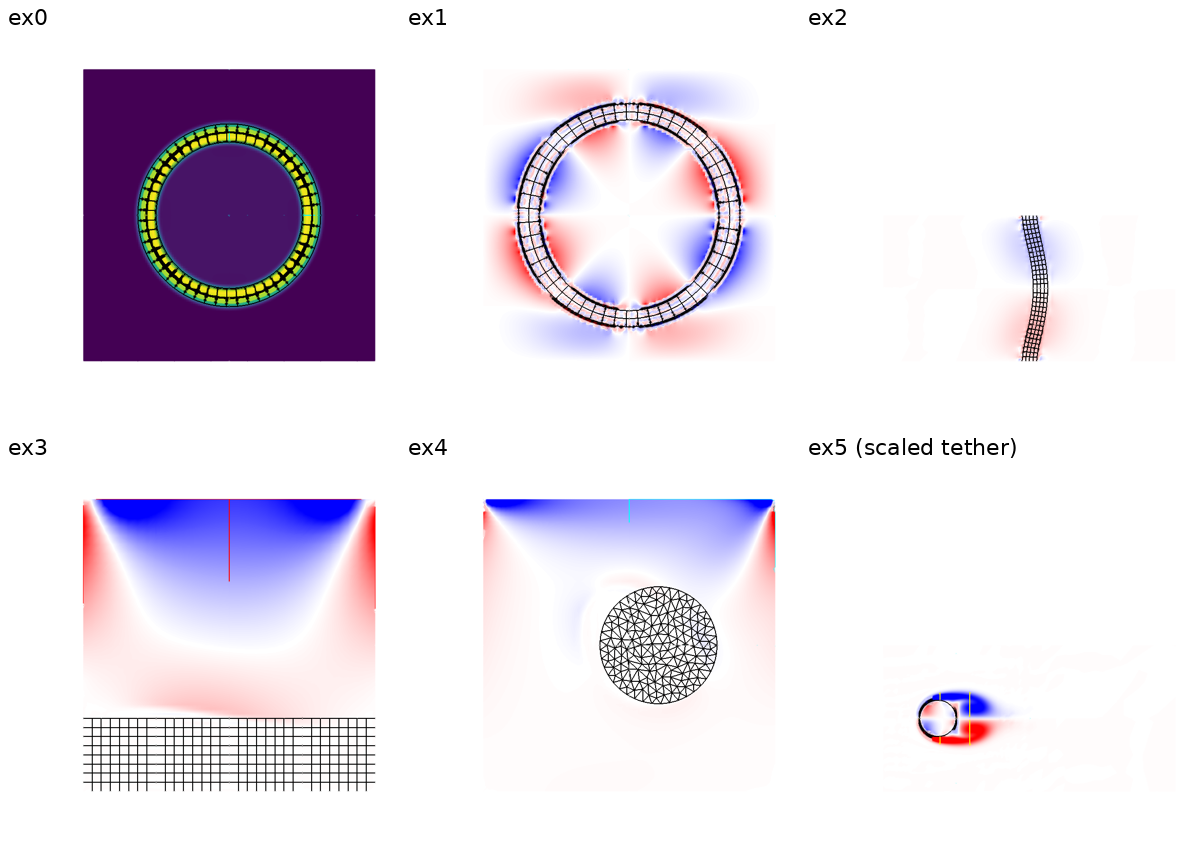
\includegraphics[height=0.7\textheight,width=0.98\textwidth,keepaspectratio]{ch25-gallery-1.png}\\
\scriptsize Vorticity (red and blue) at the last frame of each run, the bodies' meshes in black; the longer run where one exists; \code{ex0}, a static test, shows its pressure instead. Left to right, top to bottom: \code{ex0}, \code{ex1}, \code{ex2}, \code{ex3}, \code{ex4}, \code{ex5} (with the input's scaled tether, slide \ref{fr:dt2}).
\sourcecredit{IBAMR 0.19.0, four cores; \code{wsl/final/visit\_ibfe\_tour.sh}.}
\end{frame}

% 16b
\begin{frame}{Gallery (2)}
\label{fr:gallery2}
\centering
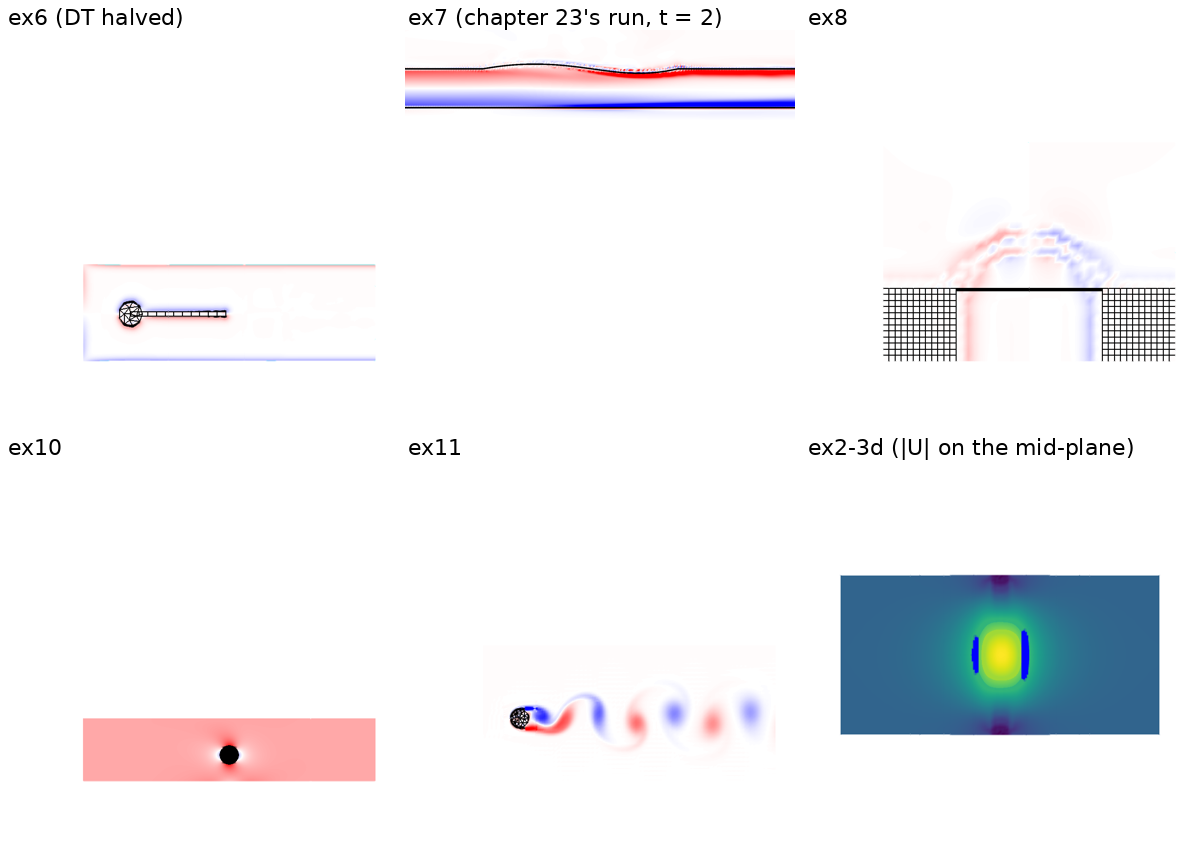
\includegraphics[height=0.72\textheight,width=0.98\textwidth,keepaspectratio]{ch25-gallery-2.png}\\
\scriptsize \code{ex6} (with \code{DT} halved, $t = 0.29$ s, the cylinder and beam end of the channel), \code{ex7} (chapter 23's run of the same example at $t = 2$; as shipped it stops at $t = 0.02$), \code{ex8}, \code{ex10} (a window round the moving cylinder), \code{ex11} (at $t = 130$, the end of the benchmark), and \code{ex2} in 3D ($|\mathbf{u}|$ on the mid-plane slice). \code{ex9} produced no frame, and the complex-fluids runs' SAMRAI dumps crash VisIt 3.5's metadata server (their \code{.curve} files are the output to read).
\end{frame}

% 17
\begin{frame}{The complex-fluids examples with bodies}
\label{fr:cf}
\footnotesize
\begin{itemize}
  \item ``These examples come from Aaron Barrett's dissertation. They are all 2D examples of complex fluids modeled using Oldroyd-B (I think). I could not get the examples with immersed boundaries to work (yet)'' (2020, slide 17). The suite is \code{examples/complex\_fluids/ex0}--\code{ex4}: a viscoelastic (Oldroyd-B) fluid solver with the polymer stress as an extra transported tensor.
  \item \al{Without bodies} (chapter 15 ran them): \code{ex0}, pipe flow with an exact solution (``error norms are printed out for the components of the conformation tensor and for the velocity''); \code{ex1}, a four-roll mill driven by a periodic body force (``as the Weissenberg number increases, singularities in the trace form at extensional points''); \code{ex3}, a lid-driven cavity with a quartic lid profile.
  \item \al{With bodies} (run for this chapter): \code{ex2}, ``flow past a confined cylinder. The structure is tethered in place using a penalty method. The structure is represented using a finite element representation following the IBFEMethod. Drag coefficients are outputted in text files. An interpolation class is included to interpolate the stress onto the surface of the cylinder'' (README); \code{ex4}, ``a four roll mill geometry with the four rollers represented by immersed structures. Rotation is imposed on the structures via a penalty method.''
\end{itemize}
\end{frame}

% 17b
\begin{frame}{The complex-fluids examples with bodies (2): why they did not work, and how they run}
\label{fr:cf2}
\footnotesize
\begin{itemize}
  \item \al{Why they did not work in 2020, and how they run now.} On four ranks both stop before the first step with a PETSc error: \code{Could not locate a solver type for factorization type ILU and matrix type mpiaij}. One of the viscoelastic solver's preconditioners asks for an incomplete LU factorization, which PETSc provides only for a matrix that lives on one rank (\code{seqaij}); on a parallel matrix (\code{mpiaij}) it needs a block-Jacobi wrapper or another preconditioner, and the shipped inputs ask for neither. On one rank (\code{mpirun -np 1}) both start and run: slide \ref{fr:table3} says how far each got in five minutes. The 2020 ``(yet)'' was almost certainly this: the course ran everything on several ranks.
  \item The IBFE side of both is Part IV's: a tethered body with \code{IBFEMethod}; what is new is the fluid, which this series does not cover beyond this slide.
\end{itemize}
\end{frame}

% 18
\begin{frame}{Where to start, for a given problem}
\label{fr:start}
\footnotesize
\begin{tabular}{@{}L{0.42\textwidth}L{0.5\textwidth}@{}}
\toprule
you want & start from \\
\midrule
a soft body deformed by a flow, no tether & \code{ex3} or \code{ex4} (and this series' IBFE/01) \\
a rigid body held in a stream, with drag and lift & \code{ex11} (direct forcing) or \code{ex5} with the solid mesh (tethers); this series' IBFE/10 for the tether version in 3D \\
a free rigid body & \code{ex10} \\
an elastic beam clamped to a rigid part & \code{ex6} (behind a cylinder) or \code{ex8} (over a slot); this series' IBFE/08 for two free parts \\
a thin membrane or shell as a surface & \code{ex5} with \code{USE\_BOUNDARY\_MESH = TRUE}, then the \code{IIM} suite \\
a body whose motion is prescribed & chapter 20's targets (volume meshes); \code{ex9}'s pattern once ported to \code{IBFESurfaceMethod} (surfaces) \\
a benchmark to validate against & \code{ex6} (Turek--Hron FSI3), \code{ex11} (cylinder at $\mathrm{Re} = 200$), \code{ex0} (exact pressure jump) \\
a scalar in the flow & this series' IBFE/12 (chapter 24), \code{IB/explicit/ex7} \\
a viscoelastic fluid round a body & \code{complex\_fluids/ex2} \\
\bottomrule
\end{tabular}

\medskip
Chapter 23's recipe reads any of them: \code{ModelData}, the \code{register} calls, the \code{getComponentDatabase} names, the mesh, the output block.
\end{frame}

% 19
\begin{frame}{What can go wrong}
\label{fr:wrong}
\scriptsize
\renewcommand{\arraystretch}{0.88}
\begin{tabular}{@{}L{0.36\textwidth}L{0.57\textwidth}@{}}
\toprule
symptom & cause and fix \\
\midrule
\code{Failed assertion: mesh->mesh\_dimension() == mesh->spatial\_dimension()} & a curve or surface mesh given to \code{IBFEMethod} (\code{ex9}); use \code{IBFESurfaceMethod} or \code{IIM}, or a volume mesh \\
\code{Time step size change encountered} & the CFL step fell below \code{dt\_max}: a tether too stiff for the step (\code{ex5}: use the input's grid-scaled \code{KAPPA\_S}) or a step too long for the body (\code{ex6}: halve \code{DT}); let the step change only to see how far it falls (slide \ref{fr:dt2}) \\
a hundred steps and the run ends & \code{END\_TIME = 100*DT}: a smoke test as shipped; raise it \\
the in-tree \code{CMakeLists.txt} fails outside the tree & it calls \code{IBAMR\_ADD\_EXAMPLE}; replace it with the six lines (slide \ref{fr:build}) \\
\code{convergence\_tester.cpp} will not link & it has its own \code{main}; leave it out of the executable \\
\code{ex7} wants \code{input2d} & it ships three cases; name one on the command line \\
the ExodusII file will not open in VisIt (\code{ex5}, 2020) & try the current build and VisIt 3.5 before blaming the file; \code{ex5} with the boundary mesh writes the surface's file \\
no picture in the gallery for a run & the run wrote no frames before its cap, or stopped (the table says which) \\
\code{ex10} takes hours & $240\,000$ steps: half an hour on four cores reaches $t = 52$ of $1200$, so the whole run is about twelve hours; \code{ex11}'s $65\,000$ steps take $27$ minutes \\
\code{complex\_fluids/ex2}, \code{ex4}: \code{PETSC ERROR ... ILU and matrix type mpiaij} & run them on one rank, or give the solver a parallel preconditioner (slide \ref{fr:cf}) \\
VisIt's metadata server crashes on a \code{dumps.visit} & seen here only for the complex-fluids runs (the extra tensor fields); read their \code{.curve} files, or try a newer VisIt \\
\bottomrule
\end{tabular}
\end{frame}

% 20
\begin{frame}{What the 2020 deck had that is now Part X}
\label{fr:legacy}
\footnotesize
\begin{tabular}{@{}L{0.46\textwidth}L{0.46\textwidth}@{}}
\toprule
2020 & now \\
\midrule
``move a Makefile and script.sh to each folder'' & the six-line \code{CMakeLists.txt}; \code{mpirun} on the laptop, \code{sbatch} on Puma (chapter 31) \\
``Make sure the Makefile has the right dimensions'' & the CMake target \code{IBAMR2d} or \code{IBAMR3d} \\
``Drop the .C / .cpp and then make'' & list only \code{example.cpp} in \code{add\_executable} \\
\code{ex2} and \code{ex8} as ``porous'' plates & a soft plate pushed by tractions; an elastic beam over a slot \\
\code{ex6} ``from a paper by Boyce'' & Turek and Hron (2006), FSI3 \\
\code{ex7} ``peristaltic transport'' & the collapsible channel of chapter 23 \\
the \code{ex5} ``.ex2 read issue'' & not reproduced with 0.19.0 and VisIt 3.5 (run table) \\
no slide for \code{ex9}; nothing after \code{ex11} & slide \ref{fr:fail}; there is nothing after \code{ex11} in 0.19.0 \\
complex-fluid IB examples ``not working (yet)'' & they need one rank (PETSc's ILU); on one rank they run (slide \ref{fr:cf}) \\
three figure crops from Griffith and Luo & own renders (gallery) \\
\bottomrule
\end{tabular}
\end{frame}

% 21
\begin{frame}{Exercises}
\label{fr:exercises}
\footnotesize
\begin{enumerate}
  \item Run \code{ex1} to $t = 0.75$ and plot the ring's area from \code{volume.curve}; compare the shape at $t = 0.75$ with Griffith and Luo's Fig.\ 4.
  \item Run \code{ex6} with \code{DT} halved to $t = 10$ (about $70\,000$ steps, half an hour on four cores at the shipped grid) and plot \code{A\_y.curve}: the FSI3 tip oscillation is about $\pm0.034$ at $5.3$ Hz once periodic.
  \item \code{ex11} for $30$ time units, then \code{compute\_St.m} (or its Python translation, chapter 33) on \code{C\_L.curve}; compare $\mathrm{St}$ and the mean $C_D$ with the published values for $\mathrm{Re} = 200$.
  \item \code{ex5} with \code{USE\_BOUNDARY\_MESH = FALSE}: does the solid disc give the same $C_D$ as the surface?
  \item \code{ex8}: plot the beam's deformed length against the pressure ramp; then double \code{MU\_S}.
  \item \code{ex10} to $t = 100$: where is the cylinder's centre, and how fast is it still moving?
  \item Port \code{ex9} to \code{IBFESurfaceMethod} (the way \code{ex5} does it) and give its velocity field a rotation.
  \item \code{ex5} in 3D: does the grid-scaled tether rescue it as it does in 2D (slide \ref{fr:dt2})? Then compare its $C_D$ with the 2D value.
  \item \code{ex6} at the shipped \code{DT} with \code{MU\_S} ten times smaller: does it run? What does that say about the limit?
\end{enumerate}
\end{frame}

% 22
\begin{frame}{Rules of thumb}
\label{fr:thumb}
\small
\begin{itemize}
  \item Read the code before the lecture note: ``I believe'' marks a guess, and the code settles it.
  \item As shipped, most IBFE examples are hundred-step smoke tests; the benchmarks are half-hour jobs on a desktop PC (\code{ex11}, \code{ex6} to a few seconds) to half a day (\code{ex10}).
  \item A curve in 2D or a surface in 3D is not an \code{IBFEMethod} body any more.
  \item ``Time step size change'' means the velocity outgrew the input: a tether too stiff or a step too long. Grid-scaled constants first, then a smaller \code{DT}; let the step adapt only to diagnose.
  \item Rigid parts: direct forcing when you want the force and the free motion, tethers when you want control.
  \item Every example writes \code{.curve} files; read them before the pictures.
\end{itemize}
\end{frame}

% 23
\begin{frame}{Summary}
\label{fr:summary}
\footnotesize
\begin{enumerate}
  \item IBAMR's twelve IBFE examples: a pressurized ring and its elliptical start, three soft bodies pushed by boundary conditions, a cylinder at $\mathrm{Re} = 200$ as a surface or a solid, the Turek--Hron beam, the collapsible channel, a clamped beam over a slot, a surface tethered to a volume's motion, and two rigid cylinders by direct forcing.
  \item They add four mechanisms to Part IV's: surface meshes with their own method, tethers that read another mesh, direct forcing for rigid bodies, and a stabilized beam.
  \item All were built standalone and run: nine run as shipped; \code{ex9} stops on the mesh-dimension assertion; \code{ex5} and \code{ex6} stop on the time-step abort, and run again with the input's own grid-scaled tether (\code{ex5}) or \code{DT} halved (\code{ex6}); the run tables give steps, times and costs.
  \item Chapter 15's one-line map was wrong and is corrected; the 2020 readings of \code{ex2}, \code{ex6}, \code{ex7} and \code{ex8} are corrected from the code.
  \item For a new problem, slide \ref{fr:start} says which example to start from and which chapter explains it.
\end{enumerate}
\begin{homebox}
\footnotesize Part IV's IBFE chapters are complete. Next: Part V, VisIt. (The horse's carotid artery, planned here as an IBFE example, became IB/13, a 2D IB example: chapter 36.)
\end{homebox}
\end{frame}

% 25
\begin{frame}{References and credits}
\label{fr:refs}
\scriptsize
\begin{itemize}
  \item IBAMR 0.19.0: \code{examples/IBFE/explicit/ex0}--\code{ex11} and \code{examples/complex\_fluids/ex0}--\code{ex4}, their inputs and READMEs; \code{src/IB/IBFEMethod.cpp}. \url{https://github.com/IBAMR/IBAMR}
  \item B. E. Griffith and X. Luo, \emph{Hybrid finite difference/finite element immersed boundary method}, Int.\ J.\ Numer.\ Meth.\ Biomed.\ Engng 33 (2017) e2888: the IBFE method and the tests \code{ex0}, \code{ex1}, \code{ex4} and \code{ex5} reproduce (its Figs.\ 4, 10, 12).
  \item S. Turek and J. Hron, \emph{Proposal for numerical benchmarking of fluid--structure interaction between an elastic object and laminar incompressible flow}, in H.-J. Bungartz and M. Sch\"afer (eds.), Fluid--Structure Interaction, Springer (2006) 371--385: \code{ex6}.
  \item A. P. S. Bhalla, R. Bale, B. E. Griffith and N. A. Patankar, \emph{A unified mathematical framework and an adaptive numerical method for fluid--structure interaction with rigid, deforming, and elastic bodies}, J.\ Comput.\ Phys.\ 250 (2013) 446--476: the direct-forcing idea behind \code{ex10} and \code{ex11}.
  \item The course material: \emph{6 -- IBFE -- What do Boyce's examples do?} (2020). The runs: \code{/root/work/0.19.0/ibfe\_tour/} (IBAMR 0.19.0, four cores); figures with VisIt 3.5.
\end{itemize}
\end{frame}

\end{document}
